\section{Цель работы}
Провести оптимизацию геометрии молекулы этиленгликоля в z-матричном представлении.

\begin{figure}[H]
\centering
\captionsetup{justification=centering}
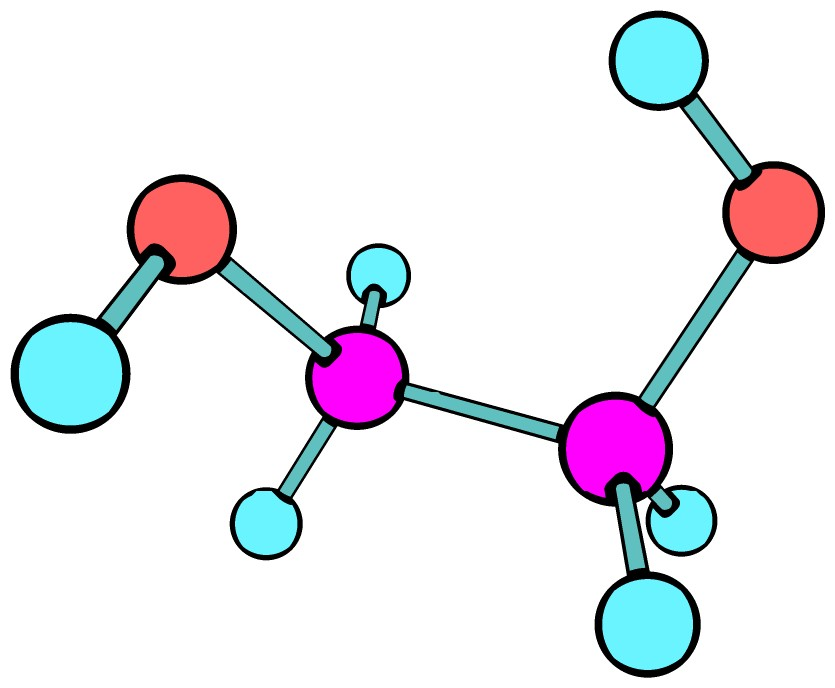
\includegraphics[scale=0.4]{fig/0.jpg}
\caption{Молекула этиленгликоля.}
\end{figure}

\newpage
\section{Постановка задачи}
Cоставить z-матрицу для молекулы этиленгликоля. Провести оптимизацию методом B3LYP в базисе 6-31G и привести следующие результаты: 
\begin{itemize}
    \item значение полной энергии и вкладов в нее до и после оптимизации;
    \item длины связей между всеми атомами, ковалентно связанными между собой;
    \item сопоставление результатов (полной энергии, длин связей, время оптимизации) со значениями, полученными в работе №2;
\end{itemize}

\newpage
\section{Теоретическая информация}
\subsection{Z-матрица}
В химии Z-матрицей называют способ представления координат атомов молекулярной системы. Кроме того, такое представление называют также внутренними координатами (internal coordinates). Это представление определяет каждый атом системы через атомный номер, длину связи, валентный угол и двугранный угол. Под связью в данном случае подразумевается не химическая связь, а просто вектор, направленный от одного атома к другому, хотя они могут и совпадать. Тем не менее, принято записывать Z-матрицу через длины и углы химических связей, так как такая запись позволяет описать не только относительное расположение атомов друг относительно друга, но и связи этих атомов.

Пример z-матрицы для молекулы этиленгликоля:
\begin{table}[H]
\resizebox{\textwidth}{!}{%
\begin{tabular}{|c|c|c|c|c|c|c|}
\hline
Element label & Atom 1 & Bond length, \AA & Atom 2 & Bond angle, \degree & Atom 3 & Dihedral angle, \degree \\ \hline
H & - & - & - & - & - &  \\ \hline
O & 1 & 1.1 & - & - & - & - \\ \hline
C & 2 & 1.2 & 1 & 109.5 & - & - \\ \hline
C & 3 & 1.4 & 2 & 109.5 & 1 & -60.9 \\ \hline
O & 4 & 1.2 & 3 & 109.5 & 2 & -60.9 \\ \hline
H & 5 & 1.1 & 4 & 109.5 & 3 & 58.6 \\ \hline
H & 3 & 1.1 & 2 & 109.5 & 1 & 60.9 \\ \hline
H & 3 & 1.1 & 2 & 109.5 & 1 & 178.9 \\ \hline
H & 4 & 1.1 & 5 & 109.5 & 6 & 179.5 \\ \hline
H & 4 & 1.1 & 5 & 109.5 & 6 & -62.6 \\ \hline
\end{tabular}%
}
\end{table}


\newpage
\section{Результаты}
\subsubsection*{Энергия системы}
Была проведена оптимизация геометрии методом B3LYP в базисе 6-31G.
\begin{table}[H]
\caption{Значения составляющих полной энергии для молекулы до и после проведения оптимизации (раздел ENERGY COMPONENTS)} \label{tab:my-table}
    \begin{center}
        \begin{tabular}{|c|c|c|}
        \hline
         & До оптимизация, Хартри & После оптимизации, Хартри \\ \hline
        \begin{tabular}[c]{@{}c@{}}Кинетическая энергия\\ электронов\end{tabular} & 230.372 & 228.911 \\ \hline
        \begin{tabular}[c]{@{}c@{}}Электрон-электронное\\ взаимодействие\end{tabular} & 227.240 & 213.149 \\ \hline
        \begin{tabular}[c]{@{}c@{}}Электрон-ядерное\\ взаимодействие\end{tabular} & -834.435 & -804.018 \\ \hline
        \begin{tabular}[c]{@{}c@{}}Ядер-ядерное\\ взаимодействие\end{tabular} & 146.936 & 131.912 \\ \hline
        \textbf{Полная энергия} & \textbf{-229.886} & \textbf{-230.045} \\ \hline
        \end{tabular}
    \end{center}
\end{table}

\subsubsection*{Длины связей}
Была проведена оптимизация геометрии методом B3LYP в базисе 6-31G.

\begin{table}[H]
\caption{Длины связей в молекуле до и после оптимизации (раздел BOND ORDER AND VALENCE ANALYSIS)}
\label{tab:tab4}
\begin{center}
\begin{tabular}{|c|c|c|c|}
\hline
\multirow{2}{*}{Связь} & \multicolumn{2}{c|}{Длина связи, \AA} & \multirow{2}{*}{\begin{tabular}[c]{@{}c@{}}Относительная \\ разница, \%\end{tabular}} \\ \cline{2-3}
 & До оптимизации & После оптимизации &  \\ \hline
O1-H9 & 1.100 & 0.980 & -10.91 \\ \hline
O1-C3 & 1.200 & 1.467 & 22.25 \\ \hline
C3-H5 & 1.100 & 1.098 & -0.18 \\ \hline
C3-H6 & 1.100 & 1.092 & -0.73 \\ \hline
C3-C4 & 1.400 & 1.523 & 8.79 \\ \hline
C4-H8 & 1.100 & 1.104 & 0.36 \\ \hline
C4-H7 & 1.100 & 1.094 & -0.55 \\ \hline
C4-O2 & 1.200 & 1.448 & 20.67 \\ \hline
O2-H10 & 1.100 & 0.983 & -10.64 \\ \hline
\end{tabular}
\end{center}{}
\end{table}

\subsubsection*{Сопоставление результатов}
В работе №2 полная энергия оптимизированный геометрии равна -230.045 Хартри. Результат, полученный в данной работе, совпадает с результатом прошлой работы. Из таблицы ниже также можно видеть, что геометрии полученных структур совпадают:
\begin{table}[H]
\caption{Сопоставление длин связей структур}
\label{tab:tab4}
\begin{center}
\begin{tabular}{|c|c|c|c|}
\hline
\multirow{2}{*}{Связь} & \multicolumn{2}{c|}{Длина связи, \AA} & \multirow{2}{*}{\begin{tabular}[c]{@{}c@{}}Относительная \\ разница, \%\end{tabular}} \\ \cline{2-3}
 & В работе №2 & В работе №4 &  \\ \hline
O1-H9 & 0.980 & 0.980 & 0.00 \\ \hline
O1-C3 & 1.467 & 1.467 & 0.00 \\ \hline
C3-H5 & 1.098 & 1.098 & 0.00 \\ \hline
C3-H6 & 1.092 & 1.092 & 0.00 \\ \hline
C3-C4 & 1.523 & 1.523 & 0.00 \\ \hline
C4-H8 & 1.104 & 1.104 & 0.00 \\ \hline
C4-H7 & 1.094 & 1.094 & 0.00 \\ \hline
C4-O2 & 1.448 & 1.448 & 0.00 \\ \hline
O2-H10 & 0.983 & 0.983 & 0.00 \\ \hline
\end{tabular}
\end{center}{}
\end{table}

Однако в предыдущей работе оптимизация сошлась за 125 сек., в то время как в данной работе -- за 165 сек.


\newpage
\section{Выводы}
Задачу оптимизации геометрии можно решать в различных координатных системах: картезианских, нормальных, картезианских масс-взвешенных, z-матричных и др. От выбора системы координат зависит скорость сходимости результата.
\newpage
\section{Контроль результатов}
Результаты данного расчета (полная энергия оптимизированной геометрии) совпадает с той, которая была получена в работе №2.
\newpage
\section{Приложенные файлы}
\begin{itemize}
    \item Ethylene\_glycol.mol – исходный файл в формате mol;
    \item Ethylene\_glycol.inp – исходные данные GAMESS для расчета методом DFT (B3LYP) в базисе 6-31G;
    \item Ethylene\_glycol.log – результат расчета методом DFT (B3LYP)  в базисе 6-31G.
\end{itemize}{}